\subsection{Definição do instrumento e do tempo}\label{sec:define_instr}

Seu início é um pequeno comentário que contêm o nome do executante e seu email para contato (primeiros sete segundos), bem como a escrita de um código que inicializa o NI-Akoustik (até 0$'$43$''$, ver \autoref{fig:SIK_piano}). 

%%%%%%%%%%%%%%%%%%%%%%%%%%%%%%%%%%%%%%%%%
\begin{example}{Definição de instrumento}
  \centering 
Primeiros eventos musicais gerados a partir das primeiras estruturas válidas de código. \textbf{Fonte}: \cite{sorensen_youtube_2014}.
  \begin{minted}[fontsize=\footnotesize]{cl}
    ;;;;;;;;;;;;;;;;;;;;;;;;;;;;;;;;;;;;;;;;;;;;;;;;;
    ;; Andrew Sorensen andrew@moso.com.au
    (define piano (au:make-node "aumu" "NaDd" "-NI-"))
    (au:connect-node piano 0 *au:output-node* 0)
    (au:update-graph)

    (au:load-preset piano "/tmp/convert_grand.aupreset")
  \end{minted}
  \label{fig:SIK_piano}
\end{example}
%%%%%%%%%%%%%%%%%%%%%%%%%%%%%%%%%%%%%%%%%


Em \tempo{0}{52} Sorensen define um tempo base. Em seguida, Sorensen apaga o código para então iniciar definições de notas (\tempo{0}{54}).

%%%%%%%%%%%%%%%%%%%%%%%%%%%%%%%%%%%%%%%%%
\begin{example}{Definição de tempo}\label{ex:def_tempo}
  \centering
  Definição do tempo base. \textbf{Fonte}: \cite{sorensen_youtube_2014}.
  \begin{minted}[fontsize=\footnotesize]{cl}
    (define *metro* (make-metro 110))
  \end{minted}
  
\end{example}
%%%%%%%%%%%%%%%%%%%%%%%%%%%%%%%%%%%%%%%%%

\subsubsection{Definição de uma sequência de blocos}

Até \tempo{1}{07}, uma rotina auxiliar é definida como um laço iterativo. Porém não encontramos sua especificação no código-fonte do Extempore.

%%%%%%%%%%%%%%%%%%%%%%%%%%%%%%%%%%%%%%%%%
\begin{example}{Definição de uma função auxiliar}
  \begin{minted}[fontsize=\footnotesize]{cl}
    (pc:cb-for-each-p chords piano
                      (pc:make-chord 50 70 2 (pc:diatonic 0 '- degree))
                      dur)
  \end{minted}
\end{example}
%%%%%%%%%%%%%%%%%%%%%%%%%%%%%%%%%%%%%%%%%

Internamente, existe uma rotina que será o cerne de execução de uma nota, acompanhada de uma lista de 4 parâmetros (50, 70, 2):

%%%%%%%%%%%%%%%%%%%%%%%%%%%%%%%%%%%%%%%%%
\begin{example}{Definição de uma nota}\label{fig:SIK_acorde}
  \begin{minted}[fontsize=\footnotesize]{cl}
(pc:make-chord 50 70 2 (pc:diatonic 0 '- degree))
  \end{minted}
\end{example}
%%%%%%%%%%%%%%%%%%%%%%%%%%%%%%%%%%%%%%%%%

A abreviação \verb|pc| significa \emph{pitch class}, e a função \verb|pc:make-chord| significa que a função cria um acorde segundo parâmetros definidos no código-fonte do \emph{Extempore}\disponivelem{https://github.com/digego/extempore/blob/master/libs/core/pc_ivl.xtm}:

\begin{citacao}
\traducao{Cria uma lista do ``número'' $[$com$]$ alturas entre limites ``menor'' e ``maior'' do \emph{pc} dado. Uma divisão dos limites, pelo número de elementos requisitados, decompõem a seleção em extensões diferentes, do qual cada altura é selecionada. \emph{make-chord} tenta selecionar alturas para todos os graus do \emph{pc}. É possível, para  os elementos de um acorde resultarem em -1, se não existir nenhum \emph{pc} para a extensão dada. $[$É$]$ não-determinístico (i.e., resultados variam com o tempo). Argumento 1: limite menor (inclusivo). Argumento 2: Limite maior (exclusivo). Argumento 3: Número de alturas no acorde. Argumento 4: \emph{pitch class} \cite{swift_playingII_2012}.}{Creates a list of "number" pitches between "lower" and "upper" bounds from the given "pc". A division of the bounds by the number of elements requested breaks down the selection into equal ranges from which each pitch is selected.  \emph{make-chord} attempts to select pitches of all degrees of the pc.  It is possible for elements of the returned chord to be -1 if no possible pc is available for the given range. Non-deterministic (i.e. result can vary each time). arg1: lower bound (inclusive).  arg2: upper bound (exclusive). arg3: number of pitches in chord.  arg4: pitch class}
\end{citacao}

Este bloco de códigos cria uma díade, no âmbito de um Ré 2 (MIDI 50) e Si bemol 3 (MIDI 70), dentro de um campo harmônico diatônico (\verb|pc:diatonic|). Por sua vez, este último cria ``um acorde seguindo regras básicas de harmonia diatônca: baseado em uma raiz (0 para C, etc.), maior/menor (\verb|'-| ou \verb|'^|) e graus (i-vii)''\footnote{Tradução nossa de: \emph{(\ldots) a chord following basic diatonic harmony rules: based on root (0 for C etc.) maj/min ('- or '\^) and degree (i-vii)}.}. O resultado não é previsível, e depende de regras específicas de qualidade, que apresentaremos adiante, para classificar os \emph{pitch class} dentro de um grau de um campo harmônico.

\subsubsection {Definição de blocos}\label{sec:define_chords}

Em \tempo{1}{08}, a função \emph{chords} surge no fluxo audiovisual, sem nenhum processo de escrita. Este comportamento caracteriza a utilização de, ou uma cópia/cola de texto, ou de uma execução de um macro do editor de texto usado. Macros são pequenos programas no editor que auxiliam o processo de produção do código. De qualquer forma é importante salientar que o código é preparado \cite{sorensen_youtube_2014}.

%%%%%%%%%%%%%%%%%%%%%%%%%%%%%%%%%%%%%%%%%%%%%%%%
\begin{example}{Algoritmo que define os acordes}

O algoritmo apresenta apenas uma propriedade, tempo (\verb|time|).

\begin{minted}[fontsize=\footnotesize]{cl}
    (define chords
       (lambda (time)
          (for-each (lambda (p)
                       (play-note (*metro* time) piano p 80 (*metro* 'dur dur)))                                 
                    (pc:make-chord 50 70 2 (pc:diatonic 0 (quote -) degree)))
          (callback (*metro* (+ time (* .5 dur))) chords (+ time dur))))

    (chords (*metro* 'get-beat 4.0) 'i 3.0)
\end{minted}
\end{example}
%%%%%%%%%%%%%%%%%%%%%%%%%%%%%%%%%%%%%%%%%%%%%%%%

Primeiro é definida a estratégia transversal, \csf{T}{ask}, com um parâmetro, \verb|time|

%%%%%%%%%%%%%%%%%%%%%%%%%%%%%%%%%%%%%%%%%%%%%%%%
\begin{example}{Estratégia transveral}
\begin{minted}[fontsize=\footnotesize]{cl}
(define chords
   (lambda (time) ... ))
\end{minted}
\end{example}

Seguido de um ``impulso'', ou um estímulo sonoro:

%%%%%%%%%%%%%%%%%%%%%%%%%%%%%%%%%%%%%%%%%%%%%%%%
\begin{example}{Impulso, ou acorde inical}
\begin{minted}[fontsize=\footnotesize]{cl}
     (chords (*metro* 'get-beat 4.0) 'i 3.0)
\end{minted}
\end{example}
%%%%%%%%%%%%%%%%%%%%%%%%%%%%%%%%%%%%%%%%%%%%%%%%

Dentro de \csf{T}{ask}, é executado um laço iterativo, \verb|for-each|, para cada nota de uma díade.

%%%%%%%%%%%%%%%%%%%%%%%%%%%%%%%%%%%%%%%%%%%%%%%%
\begin{example}{Laço iterativo}\label{sec:iterativo}
\begin{minted}[fontsize=\footnotesize]{cl}
(for-each (lambda (p)
             (play-note (*metro* time) piano p 80 (*metro* 'dur dur)))                                 
          (pc:make-chord 50 70 2 (pc:diatonic 0 (quote -) degree)))
\end{minted}
\end{example}
%%%%%%%%%%%%%%%%%%%%%%%%%%%%%%%%%%%%%%%%%%%%%%%%

Cada nota é executada com uma altura \verb|p|, para cada díade definida em \verb|pc:make-chord|, em um momento definido por \verb|time| em relação ao pulso rítmico, com uma duração ainda a ser definida. 

%%%%%%%%%%%%%%%%%%%%%%%%%%%%%%%%%%%%%%%%%%%%%%%%
\begin{example}{Execução da nota}
\begin{minted}[fontsize=\footnotesize]{cl}
(play-note (*metro* time) piano p 80 (*metro* 'dur dur))
\end{minted}
\end{example}
%%%%%%%%%%%%%%%%%%%%%%%%%%%%%%%%%%%%%%%%%%%%%%%%

\verb|play-note| é definido com os seguintes argumentos, momento de execução ($time~\Rightarrow~(*metro* time)$), o instrumento tocado, ($instr~\Rightarrow~piano$), a altura ($pitch~\Rightarrow~p$), o volume ($vol~\Rightarrow~80$) e a duração do acorde ($dur~\Rightarrow~(*metro* 'dur dur)$)\disponivelem{https://github.com/digego/extempore/blob/5aec8b35c6b3058d1c66de7abf752dc667ab61e4/libs/core/instruments-scm.xtm}. 

\subsection{Primeira sonoridade tonal}\label{sec:1aSonoridade}

Este código inicial é então modificado, e finalizado em \tempo{1}{57}, momento em que aparece uma figura, duas díades, um intervalo de quarta justa entre Sol 2 (MIDI 55) e Dó 3 (MIDI 60). entre Mi bemol 2 (MIDI 51) e Dó 3 (MIDI 60).

%%%%%%%%%%%%%%%%%%%%%%%%%%%%%%%%%%%%%%%%%%%%%%%%
\begin{example}{Estratégia transversal}
\begin{minted}[fontsize=\footnotesize]{cl}
    (define chords
       (lambda (time degree dur)
          (if (member degree '(i)) (set! dur 3.0))
          (for-each (lambda (p)
                       (play-note (*metro* time) piano p
                                  (+ 50 (* 20 (cos (* pi time))))
                                  (*metro* 'dur dur)))
                    (pc:make-chord 50 70 2 (pc:diatonic 0 (quote -) degree)))
          (callback (*metro*) (+ time (* .5 dur))) chords (+ time dur)
                    (random (assoc degree '((i vii)
                                            (vii i))))
                    dur))
    
     (chords (*metro* 'get-beat 4.0) 'i 3.0)
\end{minted}
\end{example}
%%%%%%%%%%%%%%%%%%%%%%%%%%%%%%%%%%%%%%%%%%%%%%%%

Duas transcrições desta primeira figura seguem uma estrutura literal do código, e uma perceptiva. Os primeiros eventos sonoros que ocorrem após o momento de silêncio foram transcritos antes da análise do código. Enquanto Sorensen define um tempo regular de 110 BPM  \ver{ex:def_tempo}, transcrevemos este trecho com um andamento entre 35--40 BPM \ver{fig:ask1}. É interessante notar que tais figuras simbolizam neumas \ver{fig:bipunctum}. No caso específico desta primeira figura, na mão direita, um \emph{bipunctum} , e na mão esquerda, uma \emph{clivis} \ver{fig:neumaMD1}. 

\begin{figure}[!h]
  \centering
  \input{./ask1}
  \input{./ask2}
  \caption{Transcrição literal e perceptiva do primeiro evento em \emph{A Study in Keith}. \textbf{Fonte}: autor.}
  \label{fig:ask1}
\end{figure}

 É importante notar que algumas alterações são feitas. A primeira delas é definir outros argumentos para \verb|chords|, como um acorde localizado em um grau de um campo harmônico abstrato, e a duração do acorde executado:

%%%%%%%%%%%%%%%%%%%%%%%%%%%%%%%%%%%%%%%%%%%%%%%%
\begin{example}{Modificação do código original}
\begin{minted}[fontsize=\footnotesize]{cl}
    (define chords
       (lambda (time degree dur) ...))
\end{minted}
%%%%%%%%%%%%%%%%%%%%%%%%%%%%%%%%%%%%%%%%%%%%%%%%

A segunda alteração é a indicação de uma situação condicional na primeira transformação da estratégia transversal \csf{T}{ask}. Se o grau a ser executado for uma tônica, no caso, menor \ver{sec:iterativo}, a duração deste acorde será configurada para uma duração de três unidades de tempo -- no caso da nossa transcrição, uma unidade de pulso \ver{fig:ask1}.

\begin{minted}[fontsize=\footnotesize]{cl}
(define chords
   (lambda (time degree dur)
      (if (member degree '(i)) (set! dur 3.0)) ... ))
\end{minted}

A terceira alteração modifica a intensidade das notas:

\begin{minted}[fontsize=\footnotesize]{cl}
(play-note (*metro* time) piano p
           (+ 50 (* 20 (cos (* pi time))))
           (*metro* 'dur dur))
\end{minted}

Onde a a dinâmica específica ocorre como um comportamento periódico de volumes máximos (fortes), e mínimos (pianos), em, proporcional ao cosseno do tempo instantâneo (\verb|cos (* pi time)|), escalonado para valores MIDI:

\begin{minted}[fontsize=\footnotesize]{cl}
(+ 50 (* 20 (cos (* pi time))))
\end{minted}
\end{example}

\subsubsection{Regras de qualidade}\label{sec:regras_qualidade}

A estrutura interna da estratégia \verb|chords| explicita algumas regras de qualidade, bem como permite apresentar uma primieira sequência de blocos de eventos \pressingthree{K}{ask}{0}, um conjunto de características \pressingthree{F}{ask}{0} e um pequeno grupo de objetos \pressingthree{O}{ask}{0}. Um conjunto de características é definido pelo momento de execução do evento,\pressingthree{F}{ask}{0}, o grau, \pressingthree{F}{ask}{1}, e a duração deste evento, \pressingthree{F}{ask}{2}. É importante destacar que o momento de execução é relativo ao tempo base, definido dentro do padrão \verb|* metro *| (que será explicado a seguir) de um campo harmônico, onde i representa uma tônica menor, e vii, um acorde de sétimo grau, e a duração deste acorde.

\begin{example}{Regra de qualidade \csf{R}{ask}.}
\begin{minted}[fontsize=\scriptsize]{cl}
( ... (... (callback (*metro*) (+ time (* .5 dur))) chords (+ time dur)
                    (random (assoc degree '((i vii)
                                            (vii i))))
                    dur))
\end{minted}

Cujas características irão gerar blocos de eventos, e sequências de blocos de eventos:

\begin{minted}[fontsize=\scriptsize]{cl}
( ...
  (lambda (time degree dur) ... ))
\end{minted}

O que permite executar como:
\begin{minted}[fontsize=\scriptsize]{cl}
(chords (*metro* 'get-beat 4.0) 'i 3.0)
\end{minted}
\end{example}

\subsubsection{Primeira sequência de blocos de eventos}\label{sec:primeiro_evento}

A \autoref{fig:ask3} indica uma primeira sequência de nêumas, gerados pelo algoritmo acima, em um padrão que é repetido por dois ciclos (blocos de eventos \pressingthree{E}{ask}{0} e \pressingthree{E}{ask}{1}). Durante este tempo, Sorensen realiza uma mudança (1$^o$ ciclo de bricolagem). Esta mudança transita entre o segundo bloco \pressingthree{E}{ask}{1} e terceiro bloco \pressingthree{E}{ask}{2}, e sua exeucção resulta em uma transformação da acentuação, o que termina por colocar, no último compasso deste ciclo, o sétimo grau no tempo forte e o primeiro grau no tempo fraco. 

\subsubsection*{Primeiro Bloco}

O primeiro bloco de eventos \pressingthree{E}{ask}{0} é um contraponto de primeira espécie, aticulado em tempos fortes e fracos \ver{fig:ask3}. 

\begin{figure}[!h]
  \centering
  \input{./ask3}
  \caption{Primeiros eventos musicais gerados a partir das primeiras estruturas válidas de código. \textbf{Fonte}: autor.}
  \label{fig:ask3}
\end{figure}

A aparente repetição de um mesma classe de eventos sonoros, este mesmo um objeto \pressingthree{O}{ask}{0}, pode ser diferenciada através de figuras neumáticas na mão direita e na mão esquerda \exref{fig:neumaMD1}:

\begin{example}{Transcrição de neumas do primeiro bloco}\label{fig:neumaMD1}
  Notação neumática para a um \emph{bipunctum}, dois \emph{podatus} e uma \emph{clivis} na mão direita.

  \centering{\input{./ask6}}

  E na mão esquerda, três \emph{clivis} e um bipunctum.

  \centering{\input{./ask7}}

\end{example}

\subsubsection*{Segundo Bloco}

\begin{figure}[!h]
  \centering
  \input{./ask4}
  \caption{Segundo bloco de eventos musicais. \textbf{Fonte}: autor.}
  \label{fig:ask3}
\end{figure}

Que pode ser reescrito como neumas na mão direita:

\begin{example}{Transcrição de neumas do segundo bloco}\label{fig:neumaMD2}

  Notação neumática para cinco \emph{podatus} e uma \emph{clivis} na mão direita.

  \centering{\input{./ask8}}

  E na mão esquerda uma \emph{clivis}, um \emph{podatus}, um \emph{bipunctus}, três \emph{podatus}.

  \centering{\input{./ask9}}
\end{example}

\subsubsection*{Terceiro Bloco}

Enquanto nos blocos \pressingthree{E}{ask}{0} e \pressingthree{E}{ask}{1} existem eventos significativos do ponto de vista figurativo, o aspecto rítmico é único (um tempo forte no $i$ grau, um tempo fraco na $vii$ grau). É importante destacar que, entre estes blocos, Sorensen realiza uma transformação na estratégia transversal

%%%%%%%%%%%%%%%%%%%%%%%%%%%%%%%%%%%%%%%%%%%%%%%%
\begin{example}{Primeira transformação da estratégia transversal}
\begin{minted}[fontsize=\footnotesize]{cl}
    (define chords
       (lambda (time degree dur)
          (if (member degree '(i)) (set! dur 3.0))
          (for-each (lambda (p)
                       (let* (dur1 (* dur (random '(0.5 1))))
                             (dur2 (- dur dur1)))
                       (play-note (*metro* time) piano p
                                  (+ 50 (* 20 (cos (* pi time))))
                                  (*metro* 'dur dur1))
                       (if (> dur2 0)
                           (play-note (*metro* (+ time dur1)) piano
                                      (pc:relative p (random '(-2 -1 1 2))
                                                   (pc:scale 0 'aeolian))
                                      (+ 50 (* 20 (cos (* pi (+ time dur1)))))
                                      (*metro* 'dur dur2))))
                       (pc:make-chord 50 70 2 (pc:diatonic 0 (quote -) degree)))
          (callback (*metro*) (+ time (* .5 dur)) chords (+ time dur)
                    (random (assoc degree '((i vii)
                                            (v i))))
                    (random (list 1 2 3)))))
    
     (chords (*metro* 'get-beat 4.0) 'i 3.0)
\end{minted}
\end{example}
%%%%%%%%%%%%%%%%%%%%%%%%%%%%%%%%%%%%%%%%%%%%%%%%

O que, durante esta transição, gera uma transformação na acentuação \ver{fig:ask4}.

\begin{figure}{Transcrição do terceiro bloco}
  \centering
  \input{./ask5}
  \caption{Terceiro bloco de eventos musicais. \textbf{Fonte}: autor.}
  \label{fig:ask4}
\end{figure}

Esta estratégia modifica o o laço iterativo interno de cada altura da díade:

%%%%%%%%%%%%%%%%%%%%%%%%%%%%%%%%%%%%%%%%%%%%%%%%
\begin{example}{Laço iterativo modificado}
\begin{minted}[fontsize=\footnotesize]{cl}
(for-each (lambda (p)
             (let* (dur1 (* dur (random '(0.5 1))))
                   (dur2 (- dur dur1)))
             (play-note (*metro* time) piano p
                        (+ 50 (* 20 (cos (* pi time))))
                        (*metro* 'dur dur1))
             (if (> dur2 0)
                 (play-note (*metro* (+ time dur1)) piano
                            (pc:relative p (random '(-2 -1 1 2))
                                         (pc:scale 0 'aeolian))
                            (+ 50 (* 20 (cos (* pi (+ time dur1)))))
                            (*metro* 'dur dur2))))
             (pc:make-chord 50 70 2 (pc:diatonic 0 (quote -) degree)))
\end{minted}
\end{example}
%%%%%%%%%%%%%%%%%%%%%%%%%%%%%%%%%%%%%%%%%%%%%%%%

A primeira grande mudaça é a definição de duas variáveis internas, através do comando \verb|let| (seja), chamadas \verb|dur1| e\verb|dur2|:

%%%%%%%%%%%%%%%%%%%%%%%%%%%%%%%%%%%%%%%%%%%%%%%%
\begin{example}{Laço iterativo modificado}
\begin{minted}[fontsize=\footnotesize]{cl}
(let* (dur1 (* dur (random '(0.5 1))))
                   (dur2 (- dur dur1)))
\end{minted}
\end{example}
%%%%%%%%%%%%%%%%%%%%%%%%%%%%%%%%%%%%%%%%%%%%%%%%

Estas variáveis irão tornar os ritmos de ambas as mãos independentes. O ritmo da mão direita pode ser mantido ou diminuido (\verb|(* dur (random '(0.5 1))|), enquanto o ritmo da mão esquerda é uma diferença entre uma duração geral, e o ritmo da mão direita. No caso desta nova duração da mão esquerda, é aplicado uma verificação condicional:

%%%%%%%%%%%%%%%%%%%%%%%%%%%%%%%%%%%%%%%%%%%%%%%%
\begin{example}{Laço iterativo modificado}
\begin{minted}[fontsize=\footnotesize]{cl}
(if (> dur2 0)
    (play-note (*metro* (+ time dur1)) piano
               (pc:relative p (random '(-2 -1 1 2))
                            (pc:scale 0 'aeolian))
               (+ 50 (* 20 (cos (* pi (+ time dur1)))))
               (*metro* 'dur dur2)))
\end{minted}
\end{example}
%%%%%%%%%%%%%%%%%%%%%%%%%%%%%%%%%%%%%%%%%%%%%%%%

Se a diferença entre a duração total e a nova duração for inválida (igual a $0$), o ritmo da mão esquerda será igual ao da mão direita, mas sua altura será relativa à segundas menores ou maiores ascendentes ao modo eólico da escala (que no caso transforma a sonoridade tonal em sonoridade modal). 

%%%%%%%%%%%%%%%%%%%%%%%%%%%%%%%%%%%%%%%%%%%%%%%%
\begin{example}{Laço iterativo modificado}
\begin{minted}[fontsize=\footnotesize]{cl}
(pc:relative p (random '(-2 -1 1 2))
             (pc:scale 0 'aeolian))
(+ 50 (* 20 (cos (* pi (+ time dur1)))))
\end{minted}
\end{example}
%%%%%%%%%%%%%%%%%%%%%%%%%%%%%%%%%%%%%%%%%%%%%%%%

O seu ritmo depende da duração da mão direita:

%%%%%%%%%%%%%%%%%%%%%%%%%%%%%%%%%%%%%%%%%%%%%%%%
\begin{example}{Laço iterativo modificado}
\begin{minted}[fontsize=\footnotesize]{cl}
(+ 50 (* 20 (cos (* pi (+ time dur1)))))
\end{minted}
\end{example}
%%%%%%%%%%%%%%%%%%%%%%%%%%%%%%%%%%%%%%%%%%%%%%%%

\begin{example}{Transcrição de neumas do terceiro bloco}\label{fig:neumaMD3}

  Notação neumática para um \emph{bipunctus}, uma \emph{clivis}, um \emph{porrectus subpunctis}, dois \emph{torculus}, uma \emph{clivis}  cinco \emph{podatus} e uma \emph{clivis subpunctis}, na mão direita.

  \centering{\input{./ask10}}

  E na mão esquerda, 

  \centering{\input{./ask11}}
\end{example}

E na mão esquerda:

%\begin{figure}[!h]
%  \centering
%  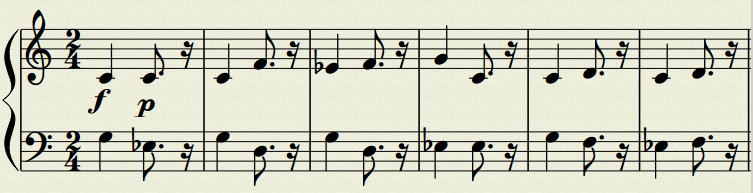
\includegraphics[scale=0.5]{imagens/SIK_motivo.png}
%  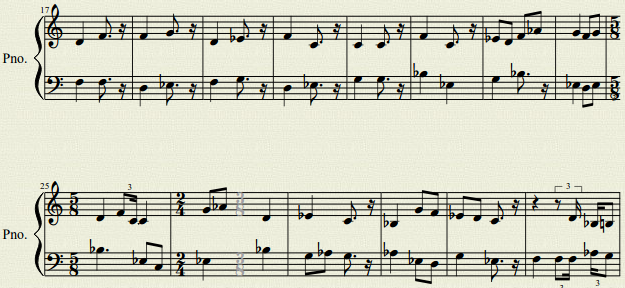
\includegraphics[scale=0.5]{imagens/SIK_perturba.png}
%  \caption{Primeiros perturbações sistêmicas. \textbf{Fonte}: autor.}
%  \label{fig:SIKinicio}
%\end{figure}

Rascunho:

\begin{figure}[!h]
  \centering
  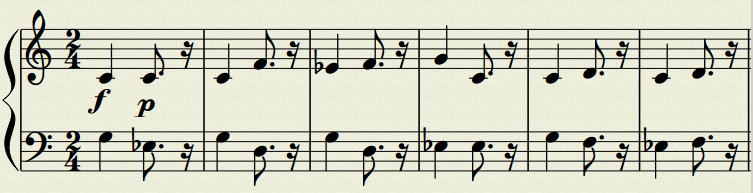
\includegraphics[scale=0.5]{imagens/SIK_motivo.png}
  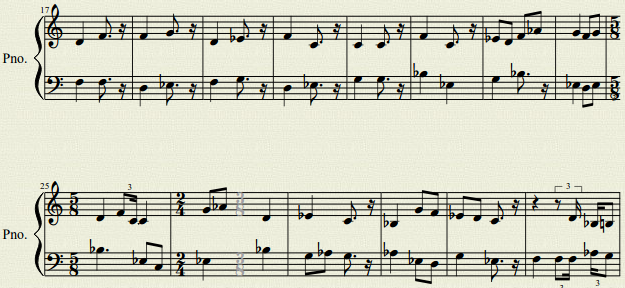
\includegraphics[scale=0.5]{imagens/SIK_perturba.png}
  \caption{Primeiros perturbações sistêmicas. \textbf{Fonte}: autor.}
  \label{fig:SIKinicio}
\end{figure}